\section{Installasi}

\subsection{Python / Anaconda}
Installasi ini pastikan sudah dikerjakan pada modul bagian Peneganalan Anaconda karena disitu sudah lengkap tutorial cara installasi dengan os ubuntu 19.04 dan windows 10.

\subsection{Chrome dan ChromeDriver}
Pastikan sudah menginstall chrome dengan versi terbaru jika sudah install periksa update dari chrome dengan cara:
\begin{enumerate}
\item mengetikkan link about chrome seperti berikut.

\begin{figure}[H]
\centerline{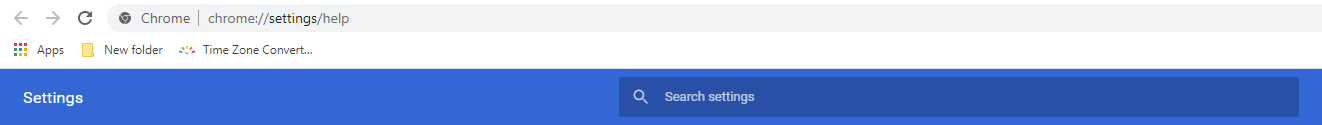
\includegraphics[scale=0.5]{figures/linkupdatechrome}}
\caption{Link About Chrome 1}
\label{linkupdatechrome}
\end{figure}

\item dengan cara mengikuti alur seperti gambar.
\begin{figure}[H]
\centerline{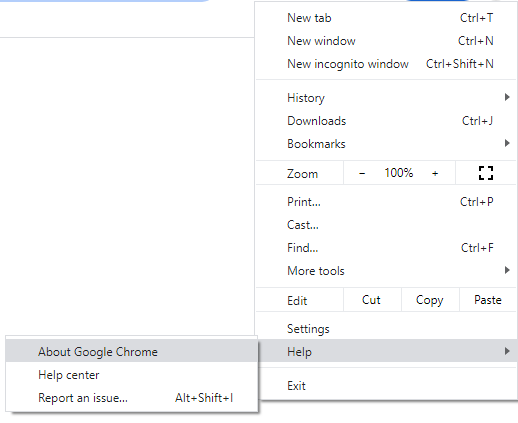
\includegraphics[scale=0.75]{figures/updatechrome}}
\caption{Link About Chrome 2}
\label{alurabout}
\end{figure}
\end{enumerate}

\section{Kodingan Wanda}
\lstinputlisting[caption=modul, language=Python, firstline=1, lastline=18]{src/chatbot.py}

\lstinputlisting[caption=getnilaiMahasiswa, language=Python, firstline=45, lastline=68]{src/chatbot.py}

\lstinputlisting[caption=cekjadwal sidang, language=Python, firstline=70, lastline=117]{src/chatbot.py}

\lstinputlisting[caption=saveProfile, language=Python, firstline=120, lastline=123]{src/chatbot.py}

\lstinputlisting[caption=splitString, language=Python, firstline=125, lastline=127]{src/chatbot.py}

\lstinputlisting[caption=waitLogin, language=Python, firstline=129, lastline=133]{src/chatbot.py}

\lstinputlisting[caption=typeAndSendMessage, language=Python, firstline=140, lastline=144]{src/chatbot.py}

\lstinputlisting[caption=deleteMessage, language=Python, firstline=146, lastline=160]{src/chatbot.py}